\documentclass[12pt]{article}
\usepackage[paperwidth=24in,paperheight=38in,margin=0in]{geometry}
\usepackage{graphicx}
\usepackage{tikz}
\usepackage{xcolor}
\usepackage{amsmath,amssymb}
\usepackage{booktabs}
\usepackage{array}
\usepackage{lmodern}
\usepackage{ragged2e}
\usepackage[T1]{fontenc}
\usepackage[final,protrusion=true,expansion=true,tracking=false]{microtype}
\setlength{\emergencystretch}{0.8em}
\hyphenpenalty=10000
\exhyphenpenalty=10000
\doublehyphendemerits=100000
\finalhyphendemerits=100000

\pagestyle{empty}
\setlength{\parindent}{0pt}
\setlength{\parskip}{0.17em}
\renewcommand{\arraystretch}{1.18}

\definecolor{primary}{RGB}{47,32,118}
\definecolor{secondary}{RGB}{0,82,145}
\definecolor{accent}{RGB}{16,130,122}
\definecolor{warning}{RGB}{176,64,55}
\definecolor{ink}{RGB}{30,34,40}
\definecolor{muted}{RGB}{83,91,104}
\definecolor{rulegray}{RGB}{198,204,214}
\definecolor{softblue}{RGB}{236,244,250}
\definecolor{softgreen}{RGB}{233,246,242}
\definecolor{softred}{RGB}{250,239,237}
\definecolor{softpurple}{RGB}{246,242,250}

\newcommand{\tightitems}{%
  \setlength{\topsep}{0.16em}%
  \setlength{\partopsep}{0pt}%
  \setlength{\itemsep}{0.30em}%
  \setlength{\parskip}{0.08em}%
  \setlength{\parsep}{0.08em}}

\newcommand{\postertextsetup}{%
  \raggedright
  \rightskip=0pt plus 2.0em
  \hyphenpenalty=10000
  \exhyphenpenalty=10000
}

\newcommand{\placeblock}[4]{%
  \node[anchor=north west, inner sep=0pt, text width=#3, align=left]
    at ([xshift=#1,yshift=-#2]current page.north west) {\postertextsetup #4};}

\newcommand{\blocktitle}[1]{%
  {\fontsize{27}{31}\selectfont\bfseries\color{primary}#1}\\[-0.01in]
  {\color{accent}\rule{\linewidth}{1.05pt}}\\[0.08in]}

\newcommand{\smalltitle}[1]{%
  {\fontsize{18.2}{23.0}\selectfont\bfseries\color{secondary}#1}\par\vspace{0.065in}}

\newcommand{\stat}[3]{%
  \begin{minipage}[t]{#1}
    {\fontsize{30}{34}\selectfont\bfseries\color{primary}#2}\\[-0.02in]
    {\fontsize{13.4}{15.8}\selectfont\color{muted}#3}
  \end{minipage}}

\newcommand{\methodbullet}[3]{%
  \textcolor{#1}{\rule{0.12in}{0.12in}}\hspace{0.08in}
  \textbf{#2}\hspace{0.055in}#3\par\vspace{0.14in}}

\newcommand{\sepline}{\vspace{0.12in}{\color{rulegray}\rule{\linewidth}{0.55pt}}\vspace{0.14in}}

\begin{document}
\begin{tikzpicture}[remember picture,overlay]
  \fill[white] (current page.south west) rectangle (current page.north east);
  \fill[primary] (current page.north west) rectangle ([yshift=-2.60in]current page.north east);
  \draw[accent,line width=1.1pt] ([yshift=-2.60in]current page.north west) -- ([yshift=-2.60in]current page.north east);
  \fill[primary] (current page.south west) rectangle ([yshift=7.10in]current page.south east);
  \draw[accent,line width=1.1pt] ([yshift=7.10in]current page.south west) -- ([yshift=7.10in]current page.south east);

  % Header
  \node[anchor=north west,text width=14.6in,align=left] at ([xshift=1.10in,yshift=-0.56in]current page.north west) {%
    {\fontsize{45}{51}\selectfont\bfseries\color{white}
    Potential-Guided Planning in Magic Tower}\\[0.08in]
    {\fontsize{23}{28}\selectfont\color{white!82}
    A deterministic long-horizon resource-allocation benchmark}\\[0.18in]
    {\fontsize{16.8}{20.5}\selectfont\bfseries\color{white}
    Bingsong Tong \quad Zhizhou Qu \quad Rui Chen}\\[0.04in]
    {\fontsize{14}{17}\selectfont\color{white!68}
    Deep Reinforcement Learning Course Project 2026}
  };

  \node[anchor=north west,text width=6.4in,align=left] at ([xshift=16.55in,yshift=-0.72in]current page.north west) {%
    {\fontsize{16.8}{20}\selectfont\bfseries\color{white}Strict replay outcomes}\\[0.08in]
    \begin{minipage}[t]{0.31\linewidth}
      {\fontsize{32}{36}\selectfont\bfseries\color{white}403}\\[-0.03in]
      {\fontsize{13}{15.5}\selectfont\color{white!68}reference HP}
    \end{minipage}\hfill
    \begin{minipage}[t]{0.31\linewidth}
      {\fontsize{32}{36}\selectfont\bfseries\color{white}315}\\[-0.03in]
      {\fontsize{13}{15.5}\selectfont\color{white!68}PUCT HP}
    \end{minipage}\hfill
    \begin{minipage}[t]{0.31\linewidth}
      {\fontsize{32}{36}\selectfont\bfseries\color{white}436}\\[-0.03in]
      {\fontsize{13}{15.5}\selectfont\color{white!68}agentic HP}
    \end{minipage}
  };

  % Compact objective strip.
  \draw[accent,line width=1.0pt] ([xshift=1.05in,yshift=-3.34in]current page.north west) -- ([xshift=23.00in,yshift=-3.34in]current page.north west);
  \placeblock{1.05in}{2.78in}{21.95in}{%
    {\fontsize{18.0}{21.8}\selectfont
    \textbf{\color{primary}Objective.}
    Magic Tower is a fully observable deterministic RPG puzzle in which legality,
    combat damage, key economy, and event flags are all exactly simulable.  We study
    whether route discovery can be improved by combining exact replay, potential-guided
    PUCT search, archive exploration, and a multi-agent reference planner.}}

  % Soft background bands for dense poster layout.
  \fill[softblue] ([xshift=1.05in,yshift=-4.28in]current page.north west) rectangle ++(6.75in,-20.05in);
  \fill[softgreen] ([xshift=8.05in,yshift=-4.28in]current page.north west) rectangle ++(7.85in,-20.05in);
  \fill[softred] ([xshift=16.15in,yshift=-4.28in]current page.north west) rectangle ++(6.85in,-20.05in);
  \draw[white,line width=8pt] ([xshift=7.94in,yshift=-4.28in]current page.north west) -- ([xshift=7.94in,yshift=-23.85in]current page.north west);
  \draw[white,line width=8pt] ([xshift=16.04in,yshift=-4.28in]current page.north west) -- ([xshift=16.04in,yshift=-23.85in]current page.north west);
  \draw[rulegray,line width=0.8pt] ([xshift=1.05in,yshift=-4.05in]current page.north west) -- ([xshift=23.00in,yshift=-4.05in]current page.north west);

  % Left band: game model.
  \placeblock{1.35in}{4.63in}{6.15in}{%
    \blocktitle{Game State as a Resource Graph}
    {\centering
      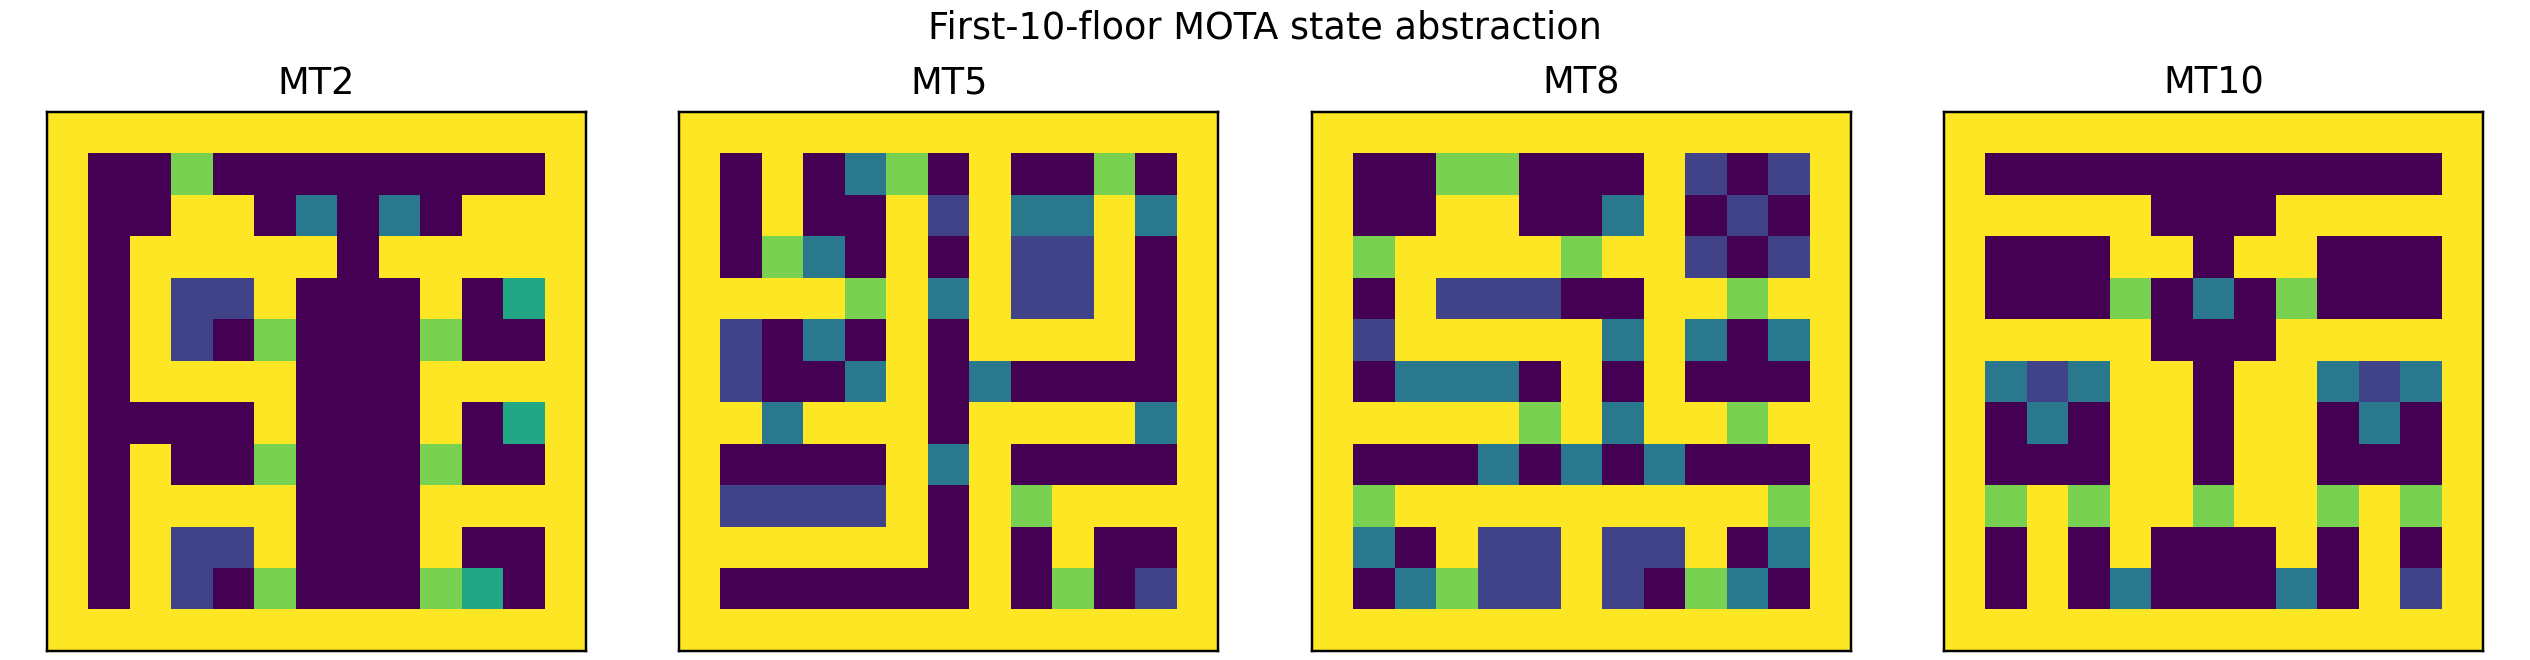
\includegraphics[width=0.99\linewidth]{../report/iclr_mota_202606/figures/mota_floor_snapshots.png}\\[-0.02in]
      {\fontsize{14.6}{19.4}\selectfont\color{muted}
      Floors expose a deterministic interaction graph: items, enemies, doors, stairs,
      merchants, and scripted events.}\par
    }\vspace{0.12in}

    \smalltitle{State and action abstraction}
    {\fontsize{17.0}{22.8}\selectfont
    \[
      \mathcal M=(\mathcal S,\mathcal A_{\mathrm{valid}},f,r,\gamma,\rho_0,\mathcal G,\mathcal F,H),
      \qquad s_{t+1}=f(s_t,a_t).
    \]
    Macro-actions select interaction nodes; walking and floor transfer paths are
    internal to the transition function.}

    \sepline

    \smalltitle{Combat threshold}
    {\fontsize{17.0}{22.8}\selectfont
    \[
      C(s,e)=
      \left\lceil\frac{\mathrm{HP}_e}
      {\max(1,\mathrm{ATK}(s)-\mathrm{DEF}_e)}\right\rceil
      \max(0,\mathrm{ATK}_e-\mathrm{DEF}(s)).
    \]
    A single ATK or DEF point can sharply reduce future damage, so reward and value
    estimates must represent marginal threshold effects.}

    \sepline

    \smalltitle{Fast executable mask}
    {\fontsize{16.9}{22.7}\selectfont
    The planner first computes the set of executable interaction nodes, then calls the
    simulator only for selected transitions.
    \begin{itemize}\tightitems
      \item Static topology and interaction coordinates are precomputed once.
      \item Dynamic doors, defeated enemies, and consumed resources are encoded as
      compact blocker bitsets.
      \item Paths are recovered lazily only for the chosen macro-action.
    \end{itemize}}

    \sepline

    \smalltitle{MOTA-specific challenge}
    {\fontsize{16.6}{22.3}\selectfont
    \begin{itemize}\tightitems
      \item \textbf{Irreversible resource use:} keys, potions, and combat losses can make
      a much later floor infeasible.
      \item \textbf{Threshold combat:} one ATK or DEF point can change multiple future
      enemy losses discontinuously.
      \item \textbf{Hybrid state:} spatial topology, consumed map nodes, hero scalars,
      and event flags must be evaluated jointly.
    \end{itemize}}

    \smalltitle{Planner features}
    {\fontsize{16.2}{21.9}\selectfont
    Hero resources, consumed-node bitsets, legal masks, missing keys, path length,
    current enemy damage, ATK+1/DEF+1 damage drops, boss margin, and unlocked
    resource value.}\\[0.20in]

    {\fontsize{18.4}{22.1}\selectfont\bfseries\color{primary}
    Core abstraction}\\[0.04in]
    {\fontsize{16.9}{22.7}\selectfont
    The agent does not choose arrow keys. It chooses the next meaningful interaction
    node, while the simulator deterministically executes the shortest legal path.}

    \sepline

    \smalltitle{State signature}
    {\fontsize{16.5}{22.3}\selectfont
    \begin{itemize}\tightitems
      \item \textbf{Hero inventory:} HP, ATK, DEF, money, and three key counts.
      \item \textbf{Map memory:} consumed resources, defeated enemies, opened doors,
      and event flags.
      \item \textbf{Frontier information:} executable nodes, masked nodes, missing
      keys, damage margins, and newly unlocked resources.
    \end{itemize}}

    \vspace{0.05in}
    \smalltitle{Why graph actions help}
    {\fontsize{16.5}{22.8}\selectfont
    The action space becomes the set of currently meaningful resource interactions,
    so search effort is spent on route choices rather than on repeated corridor
    movement.}
  }

  % Middle band: methods and search loop.
  \placeblock{8.35in}{4.63in}{7.25in}{%
    \blocktitle{Potential-Guided Planning Loop}
    {\centering
      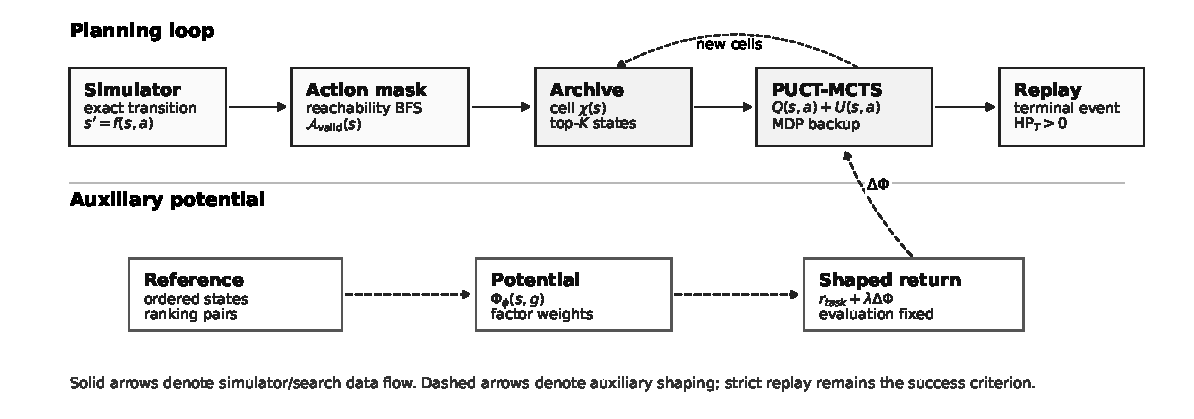
\includegraphics[width=1.00\linewidth]{../report/iclr_mota_202606/figures/system_diagram.pdf}\\[0.14in]
      {\fontsize{14.6}{19.4}\selectfont\color{muted}
      The search loop uses exact simulator transitions, legal action masks, archive cells,
      PUCT rollouts, and strict replay validation.}\par
    }\vspace{0.18in}

    \smalltitle{Complementary approaches}
    {\fontsize{16.6}{22.4}\selectfont
    \methodbullet{secondary}{Reference-route construction.}{Ordered successful states
    validate the simulator and support progress estimation.}
    \methodbullet{accent}{AlphaGo Zero-style planning.}{Policy/value priors guide
    single-agent PUCT-MCTS over macro-actions.}
    \methodbullet{warning}{Agentic planner.}{Multiple scoring modules evaluate the same
    candidate after-states, while a beam arbiter keeps legal transitions.}}

    \sepline

    \smalltitle{Potential-based shaping}
    {\fontsize{16.8}{22.7}\selectfont
    \[
      r_{\mathrm{search}}=
      r_{\mathrm{task}}+\lambda\left[\gamma\Phi_\phi(s',g')-\Phi_\phi(s,g)\right].
    \]
    \[
      \mathcal L_\Phi=
      -\sum_{(s^+,s^-)}\log\sigma(\Phi_\phi(s^+,g^+)-\Phi_\phi(s^-,g^-)).
    \]
    The shaped reward guides search and ranking; strict terminal replay remains the
    evaluation objective.}\\[0.05in]
    {\centering
      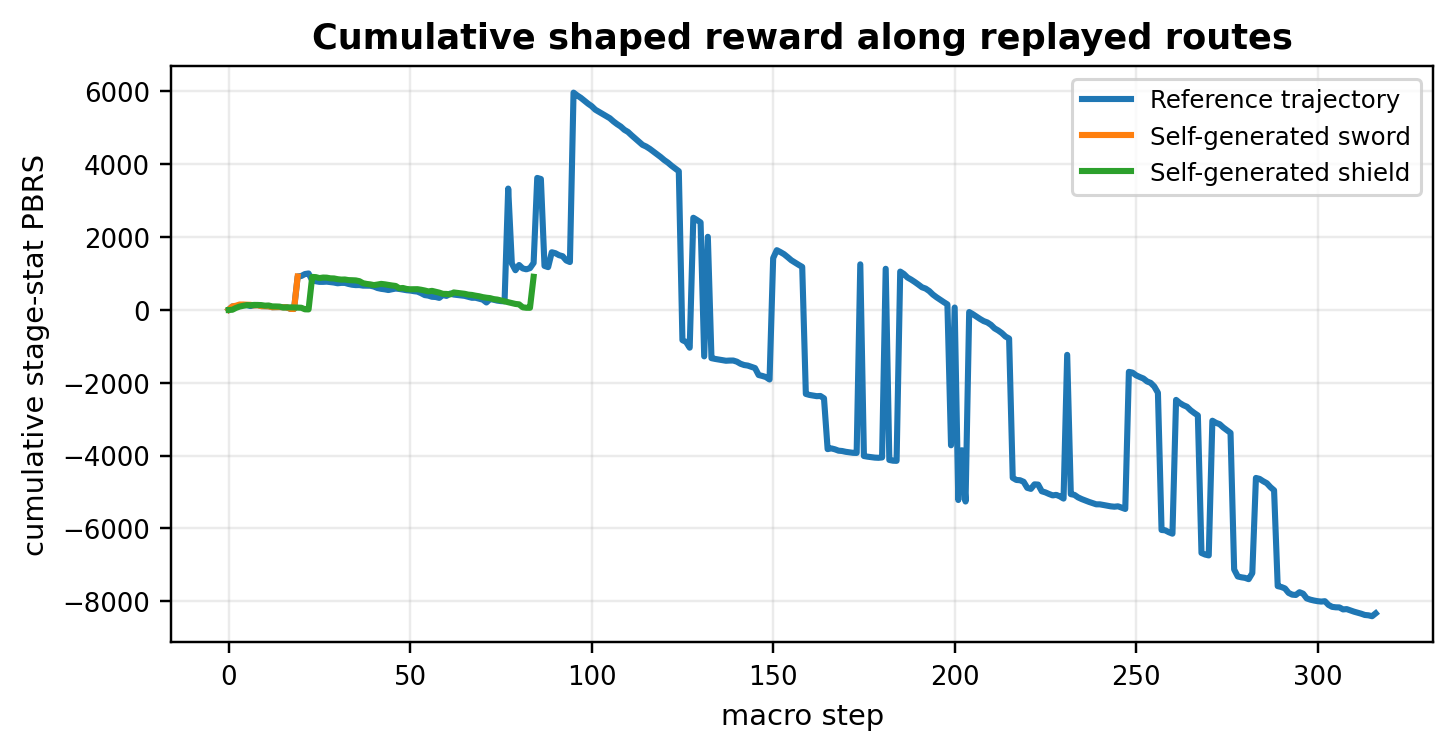
\includegraphics[width=0.93\linewidth]{../report/iclr_mota_202606/figures/reward_curves.png}\par
    }\vspace{0.10in}

    \smalltitle{Agentic reference planner}
    {\centering
      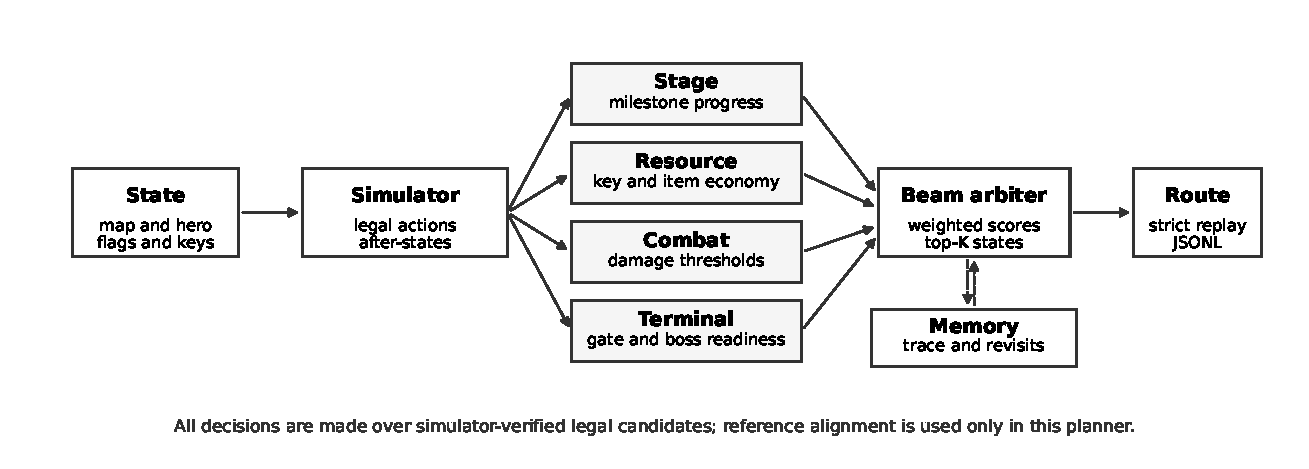
\includegraphics[width=0.98\linewidth]{../report/iclr_mota_202606/figures/agentic_architecture.pdf}\par
    }

    \sepline

    \smalltitle{Archive-guided local search}
    {\fontsize{15.8}{21.6}\selectfont
    \[
      \mathcal B[\chi(s)] = \text{top-}K\text{ non-dominated states in an abstract cell}.
    \]
    Each iteration selects a promising archive cell, restores its simulator state,
    runs short PUCT rollouts, and inserts newly reached states by lexicographic score:
    \[
      (\mathbf 1[\text{success}],\,\text{stage progress},\,\mathrm{HP},\,\text{keys},\,-\text{depth}).
    \]
    \[
      \chi(s)=
      (g,\mathrm{floor},\mathrm{ATK}_{bin},\mathrm{DEF}_{bin},
      \mathrm{keys}_{bin},\mathrm{HP}_{bin},\mathrm{boss}_{bin}).
    \]
    }\\[0.10in]
    {\fontsize{18.4}{22.1}\selectfont\bfseries\color{primary}
    Search principle}\\[0.04in]
    {\fontsize{16.8}{22.6}\selectfont
    The archive preserves alternative resource schedules; MCTS then spends local
    computation near promising but not yet solved intermediate states.}
  }

  % Right band: empirical evidence.
  \placeblock{16.40in}{4.63in}{6.35in}{%
    \blocktitle{Evidence From Strict Replay}
    {\centering
      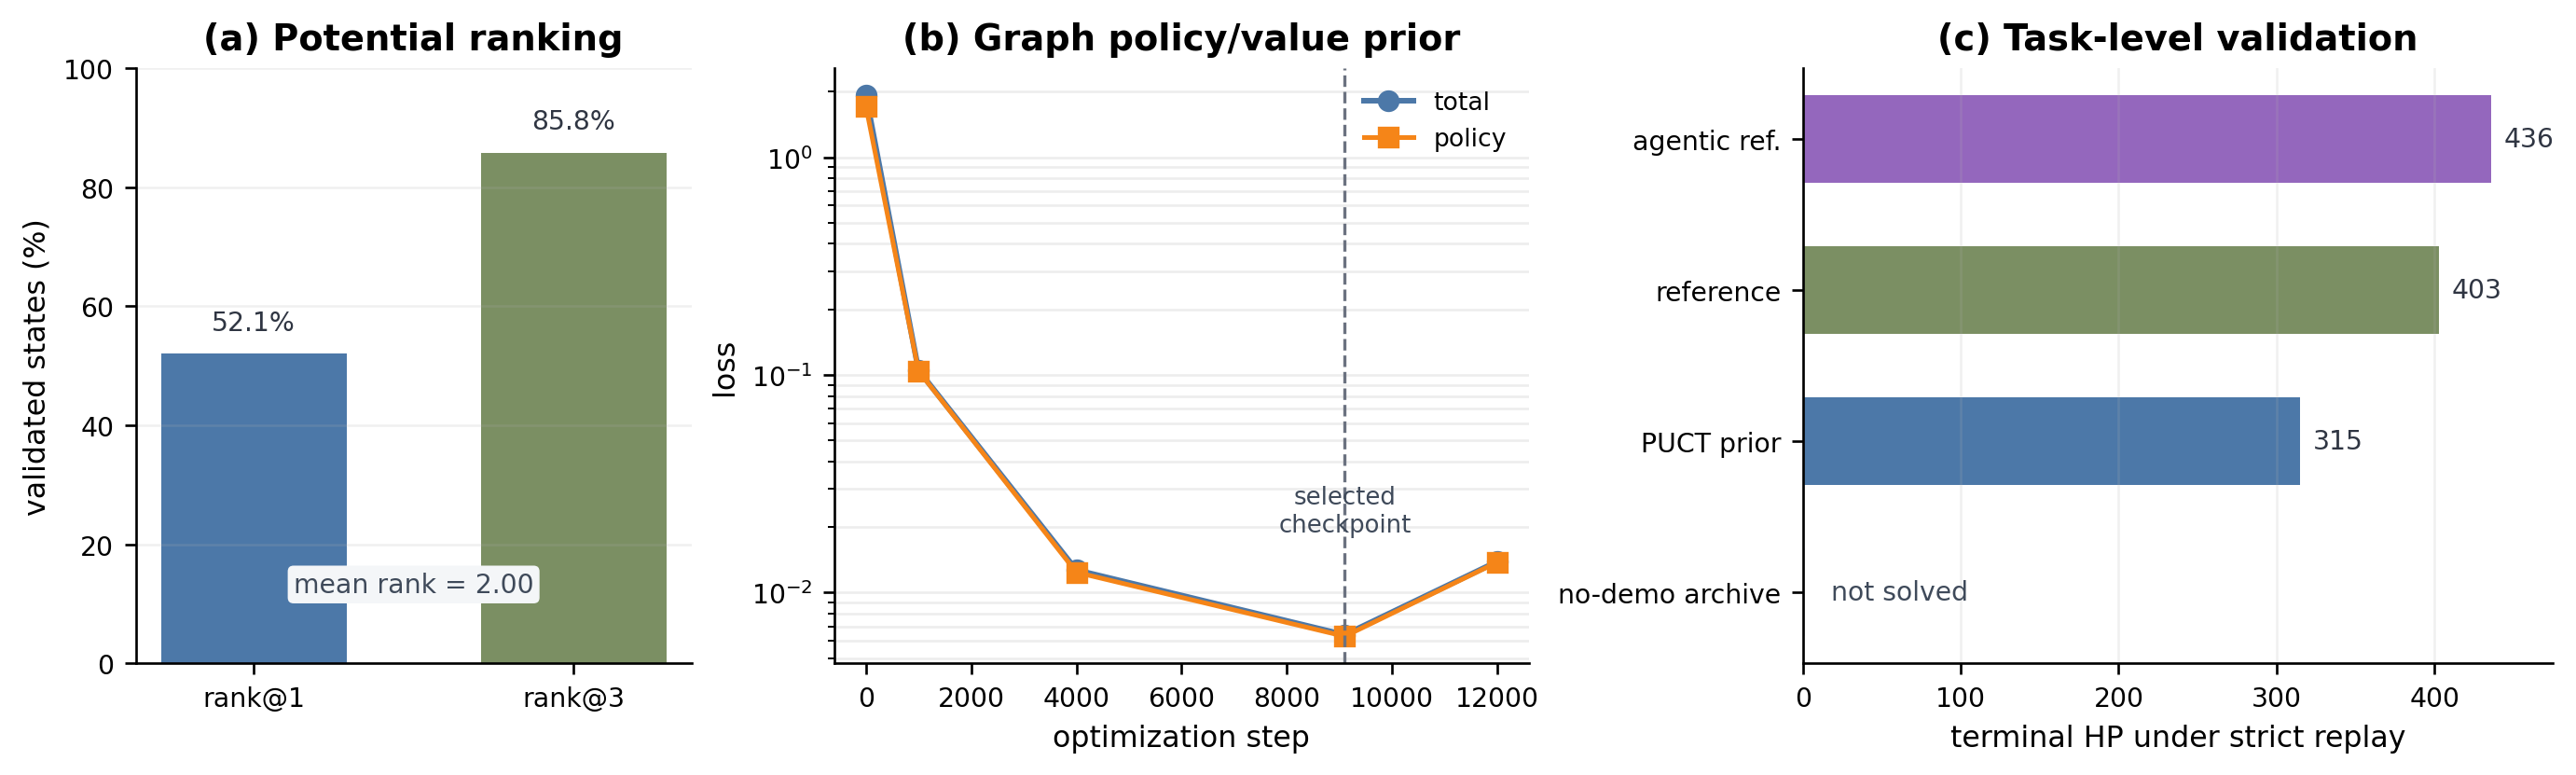
\includegraphics[width=1.00\linewidth]{../report/iclr_mota_202606/figures/experiment_summary.png}\\[-0.01in]
      {\fontsize{14.6}{19.4}\selectfont\color{muted}
      Potential ranking, policy/value fitting, and strict replay results are evaluated
      separately.}\par
    }\vspace{0.16in}

    {\fontsize{17.0}{22.8}\selectfont
    Strict replay confirms that all reported successful routes reach the terminal
    encounter with positive HP; the best multi-agent route improves the reference
    terminal margin.}\\[0.14in]

    \smalltitle{Route structure}
    {\centering
      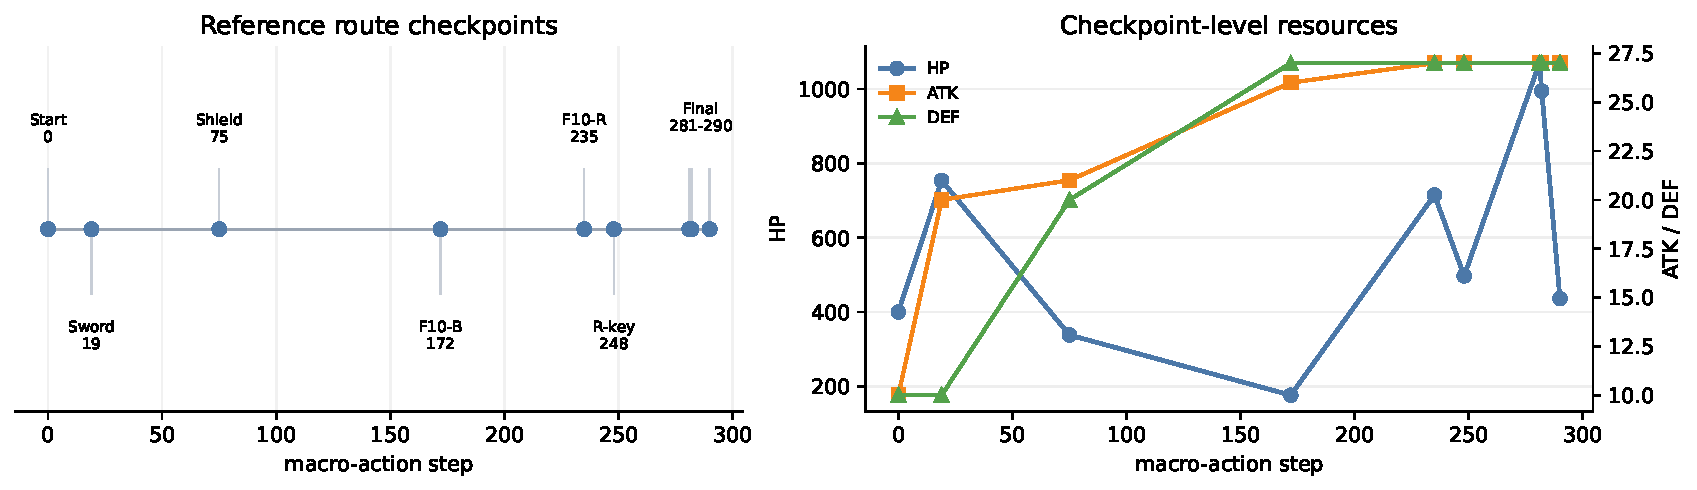
\includegraphics[width=1.00\linewidth]{../report/iclr_mota_202606/figures/agentic_route_summary.pdf}\\[0.08in]
      {\fontsize{14.6}{19.4}\selectfont\color{muted}
      Successful play accepts controlled HP losses to acquire equipment and stat resources,
      then rebuilds terminal HP margin.}\par
    }

    \sepline

    \smalltitle{Single-agent PUCT backup}
    {\fontsize{16.3}{22.0}\selectfont
    \[
      G_k=\sum_{i=k}^{L-1}\gamma^{i-k}r_{\mathrm{search}}(s_i,a_i,s_{i+1})
      +\gamma^{L-k}\hat V(s_L).
    \]
    \[
      a=\arg\max_a Q(s,a)+c_{\mathrm{puct}}P_\theta(a\mid s)
      \frac{\sqrt{\sum_b N(s,b)}}{1+N(s,a)}.
    \]}

    \vspace{0.02in}
    {\fontsize{15.7}{20.8}\selectfont
    \begin{tabular}{@{}p{1.75in}p{1.00in}p{2.55in}@{}}
      \textbf{\color{secondary}Condition} & \textbf{\color{secondary}HP} & \textbf{\color{secondary}Interpretation}\\
      \hline
      Reference route & 403 & simulator and potential-factor validation\\
      PUCT prior & 315 & closed-loop search reaches terminal event\\
      Agentic planner & 436 & stronger reference trajectory under strict replay\\
      No-demo archive & -- & reaches milestones but not terminal success\\
    \end{tabular}}

    \sepline

    \smalltitle{Evaluation discipline}
    {\fontsize{16.4}{22.2}\selectfont
    \begin{itemize}\tightitems
      \item Strict replay is the validity criterion; shaped return is never counted as
      success.
      \item The potential model uses ordered successful states only as a dense search
      signal.
      \item Pure archive search is reported separately from the multi-agent reference
      planner; model confidence never replaces simulator replay.
    \end{itemize}}

    \smalltitle{Observed bottlenecks}
    {\fontsize{16.4}{22.2}\selectfont
    Premature combat, key starvation, early potion use, local loops, and insufficient
    terminal HP explain most failed strict replays.}\\[0.20in]

    \smalltitle{What the traces show}
    {\fontsize{16.5}{22.3}\selectfont
    \begin{itemize}\tightitems
      \item Successful routes delay many combats until equipment and stat thresholds
      reduce deterministic losses.
      \item Key economy and terminal HP margin remain the binding constraints near
      the final encounter.
    \end{itemize}}
  }

  % Dense bottom benchmark panel on white area.
  \draw[rulegray,line width=0.8pt] ([xshift=1.05in,yshift=-24.35in]current page.north west) -- ([xshift=23.00in,yshift=-24.35in]current page.north west);
  \placeblock{1.05in}{24.75in}{21.95in}{%
    \blocktitle{Benchmark Extension: Text, Video, and Symbolic Control}
    \begin{minipage}[t]{0.30\linewidth}
      \vspace{0pt}
      {\fontsize{17.2}{23.2}\selectfont
      \smalltitle{Agent-facing interface}
      A MOTA instance can be exposed as synchronized symbolic, textual, and visual
      observations while preserving exact transition validation.\\[0.08in]
      Symbolic state, action masks, text prompts, and rendered route videos can be
      generated from the same deterministic transition log.\\[0.12in]
      \smalltitle{Why this benchmark scales}
      Community tower archives contain many hand-designed maps and play traces; these
      support both supervised pretraining and strict out-of-distribution evaluation.}
    \end{minipage}\hfill
    \begin{minipage}[t]{0.37\linewidth}
      \vspace{0pt}
      {\fontsize{17.2}{23.2}\selectfont
      \smalltitle{Benchmark protocol}
      \begin{tabular}{@{}p{1.45in}p{5.85in}@{}}
        \textbf{\color{secondary}Input} &
        symbolic state, text description, legal macro-actions, or rendered video.\\[0.05in]
        \textbf{\color{secondary}Action} &
        choose one legal interaction node; the simulator executes the deterministic path.\\[0.05in]
        \textbf{\color{secondary}Validity} &
        exact replay under the transition log, not model confidence or shaped return.\\[0.05in]
        \textbf{\color{secondary}Quality} &
        terminal success, terminal HP, route length, and transfer to modified towers.
      \end{tabular}\\[0.12in]
      This protocol connects symbolic planning, language-conditioned control, and
      video-based agent evaluation without changing the underlying transition
      function.}
    \end{minipage}\hfill
    \begin{minipage}[t]{0.28\linewidth}
      \vspace{0pt}
      {\fontsize{17.2}{23.2}\selectfont
      \smalltitle{Evaluation axes}
      Validity is exact replay; quality is terminal HP and route length; coverage is
      the number of distinct milestone schedules; learning is transfer across modified
      maps and unseen towers.\\[0.12in]
      \smalltitle{Open bottlenecks}
      \begin{itemize}\tightitems
        \item sparse terminal reward under-covers late key and HP schedules;
        \item potential learning improves progress ranking, but cannot replace archive diversity;
        \item text/video agents must explain both legality and long-horizon resource trade-offs.
      \end{itemize}}
    \end{minipage}
  }

  % Bottom conclusion panel.
  \placeblock{1.10in}{31.20in}{21.80in}{%
    {\fontsize{27}{33}\selectfont\bfseries\color{white}Takeaways and released artifacts}\\[-0.01in]
    {\color{accent}\rule{\linewidth}{1.0pt}}\\[0.20in]
    \begin{minipage}[t]{0.33\linewidth}
      {\fontsize{21}{26}\selectfont\bfseries\color{white}Exactness first}\\[0.07in]
      {\fontsize{16.2}{22.8}\selectfont\color{white!84}
      All reported routes are checked by deterministic replay, so terminal HP, key
      balances, defeated enemies, and event flags are auditable rather than inferred
      from model score.}
    \end{minipage}\hfill
    \begin{minipage}[t]{0.33\linewidth}
      {\fontsize{21}{26}\selectfont\bfseries\color{white}Learning as guidance}\\[0.07in]
      {\fontsize{16.2}{22.8}\selectfont\color{white!84}
      The potential model supplies dense progress information for PUCT and archive
      priority; the terminal objective remains strict replay success with positive HP.}
    \end{minipage}\hfill
    \begin{minipage}[t]{0.29\linewidth}
      {\fontsize{21}{26}\selectfont\bfseries\color{white}Benchmark trajectory}\\[0.07in]
      {\fontsize{16.2}{22.8}\selectfont\color{white!84}
      The same environment supports symbolic agents, language-conditioned agents,
      and video-based agents over a shared replayable action interface.}
    \end{minipage}\\[0.28in]
    {\color{white!28}\rule{\linewidth}{0.55pt}}\\[0.17in]
    {\fontsize{16.5}{23.0}\selectfont\color{white!88}
    \textbf{Transition log schema:}\quad
    checksum \(\rightarrow\) action mask \(\rightarrow\) interaction node
    \(\rightarrow\) combat/key/event update \(\rightarrow\) potential factors
    \(\rightarrow\) strict replay verdict.}\\[0.28in]
    \begin{minipage}[t]{0.19\linewidth}
      {\fontsize{18.8}{23.0}\selectfont\bfseries\color{white}Simulator}\\[0.01in]
      {\fontsize{14.4}{19.4}\selectfont\color{white!66}deterministic rules}
    \end{minipage}\hfill
    \begin{minipage}[t]{0.19\linewidth}
      {\fontsize{18.8}{23.0}\selectfont\bfseries\color{white}Graph state}\\[0.01in]
      {\fontsize{14.4}{19.4}\selectfont\color{white!66}all-node action mask}
    \end{minipage}\hfill
    \begin{minipage}[t]{0.19\linewidth}
      {\fontsize{18.8}{23.0}\selectfont\bfseries\color{white}PUCT-MCTS}\\[0.01in]
      {\fontsize{14.4}{19.4}\selectfont\color{white!66}policy-value search}
    \end{minipage}\hfill
    \begin{minipage}[t]{0.19\linewidth}
      {\fontsize{18.8}{23.0}\selectfont\bfseries\color{white}Potential}\\[0.01in]
      {\fontsize{14.4}{19.4}\selectfont\color{white!66}progress shaping}
    \end{minipage}\hfill
    \begin{minipage}[t]{0.19\linewidth}
      {\fontsize{18.8}{23.0}\selectfont\bfseries\color{white}Visualizer}\\[0.01in]
      {\fontsize{14.4}{19.4}\selectfont\color{white!66}text-video replay}
    \end{minipage}\\[0.28in]
    {\fontsize{15.2}{21.0}\selectfont\color{white!78}
    \textbf{Artifacts:} simulator, macro-action environment, graph-state encoder,
    potential training logs, archive cells, trajectory logs, failure cases, route
    visualizer, and report figures.}
  }

  \node[anchor=south west,text width=21.80in,align=left]
    at ([xshift=1.10in,yshift=1.55in]current page.south west) {%
    {\fontsize{21.5}{27.0}\selectfont\bfseries\color{white}
    Central claim: exact symbolic replay gives a hard success criterion, while
    potential-guided PUCT and archive search provide scalable guidance for long-horizon
    resource planning.}};

\end{tikzpicture}
\end{document}
